\documentclass[../thesis.tex]{subfiles}
\begin{document}
\chapter{Literature Review}\label{cap:literature_review}
Serverless frameworks and the web crawling process are continuously growing areas of research. The latter is a more mature field: the first web crawlers appeared in 1994 \cite{article:history_web_crawler_2014}, and they have taken advantage of the latest technologies. On the other hand, the serverless paradigm is a relatively younger technology: the first serverless platform was introduced at the end of 2014 by \acrshort{AWS} and it was called \acrshort{AWS} Lambda \cite{site:introducing_aws_lambda}.
Both fields are characterized by many publications documenting issues, challenges and innovations. This section will describe some examples of publications about these two topics.

Hongfei Yan et al. designed and evaluated an efficient web crawling system \cite{article:design_evaluation_efficient_crawler_2002} where they implemented a fully distributed web crawler, a \acrshort{URL} allocation algorithm and a method to ensure the scalability of the system. It includes a \acrfull{WSR} that manages several main controllers; each main controller coordinates its own collector, which performs the crawling process. To improve communication performance, only \acrshort{URL}s are shared. Another similar system is shown in \cite{article:ubi_distributed_crawler_2004}, where the authors implemented a scalable and fully distributed web crawler using the Java programming language. Thanks to this choice, the software can be platform-independent. It consists of multiple identically programmed agents that communicate with each other to crawl the web, ensuring dynamic and decentralized coordination between them. To avoid overloading individual agents, the amount of \acrshort{URL} to be handled by each of them is equally distributed.

Two cloud-based web crawlers are discussed in \cite{inproceedings:cloud_based_crawler_2015} and \cite{inproceedings:cloud_web_scraping_2017}, where services provided by Azure and \acrshort{AWS} are used respectively. The first exploits the MapReduce programming paradigm and uses distributed agents, each of which stores what it finds on Azure Tables or Blobs\footnote{Azure Table is a NoSQL store of key-values for rapid development while Azure Blob allows massive storage of unstructured data. Both are storage services provided by Azure. See \href{https://azure.microsoft.com/en-us/products/storage/tables}{https://azure.microsoft.com/en-us/products/storage/tables} and \href{https://azure.microsoft.com/en-us/products/storage/blobs}{https://azure.microsoft.com/en-us/products/storage/blobs} for more details.}. The second makes use of various \acrshort{AWS} services such as \acrshort{EC2}, \gls{dynamo_db}, \acrshort{SQS} and \acrshort{S3} to perform on-demand web scraping for big data applications. To understand better how this last solution works, the architecture is shown in \autoref{fig:cloud_crawler_aws}.

\begin{figure}[H]
    \centering
    \begin{subfigure}[t]{.45\textwidth}
        \centering
        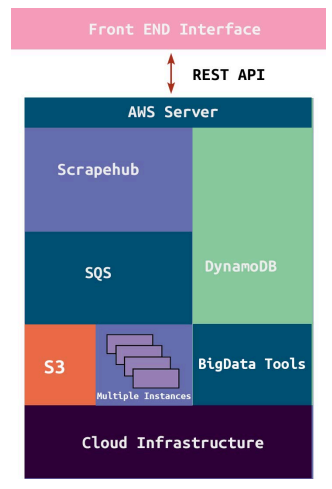
\includegraphics[width=.9\linewidth]{literature_review/cloud_crawler_aws_architecture.png}
        \caption{Ecosystem.}
        \label{fig:cloud_crawler_aws_architecture}
    \end{subfigure}
    \hfill
    \begin{subfigure}[t]{.45\textwidth}
        \centering
        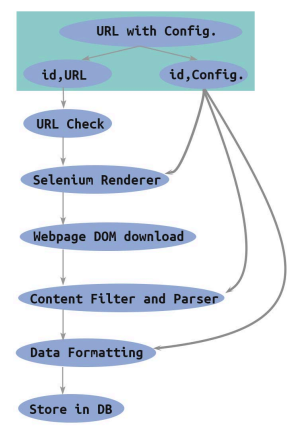
\includegraphics[width=.9\linewidth]{literature_review/cloud_crawler_aws_logic.png}
        \caption{Engine.}
        \label{fig:cloud_crawler_aws_logic}
    \end{subfigure}
    \caption[Example of cloud-based web scraper architecture]{Diagrams show the architecture and logic workflow of a cloud-based web scraper. Users request the scraping service through a \acrshort{UI}, providing URLs and configurations. These are stored in a database in \acrshort{JSON} format, and a request is generated in \acrshort{SQS} by Scrapehub. The engine reads the \acrshort{URL}s and configuration from the \acrshort{JSON} file, checks the validity of the \acrshort{URL}s, renders the valid ones using a Selenium Renderer, and stores the extracted content in the database after parsing and filtering. Pictures from \citetitle{inproceedings:cloud_web_scraping_2017} \cite{inproceedings:cloud_web_scraping_2017}.}
    \label{fig:cloud_crawler_aws}
\end{figure}

Other solutions that aim to implement a web crawler/scraper exploiting \acrshort{AWS} Lambda serverless service are illustrated in \cite{site:aws_serverless_web_scraping_2020} and \cite{site:aws_serverless_crawler_engine_2021}. In the first, some considerations are made regarding the different implementations that can be put in place to implement a web scraper, from an on-premises-like solution to a serverless solution.

\begin{itemize}
    \item Use an \acrshort{EC2} instance to have full control of the infrastructure. It requires manual operations, such as setting up the environment, completing security tasks and monitoring the health status over time;
    \item Containerise the application and deploy it on \acrlong{ECS}. The biggest advantage of this is the platform independence;
    \item Use a Lambda serverless service, which allows a very lean infrastructure to be created on demand and scales continuously, with a generous free monthly tier. The main constraint of this is that the execution time of each individual function is limited to 15 minutes.
\end{itemize}

In the second, a serverless web crawler with a search engine was developed not only using \acrshort{AWS} Lambda but also \gls{dynamo_db}, \gls{step_funcs}, \acrshort{S3} and \gls{kendra} services. \autoref{fig:aws_crawler_search_engine} shows how these components interact, making it possible to run several crawlers simultaneously that store the title text and \acrshort{HTML} text of the processed pages, with the aim of performing keyword searches on \gls{kendra}.

\begin{figure}[H]
    \centering
    \begin{subfigure}[t]{.9\textwidth}
        \centering
        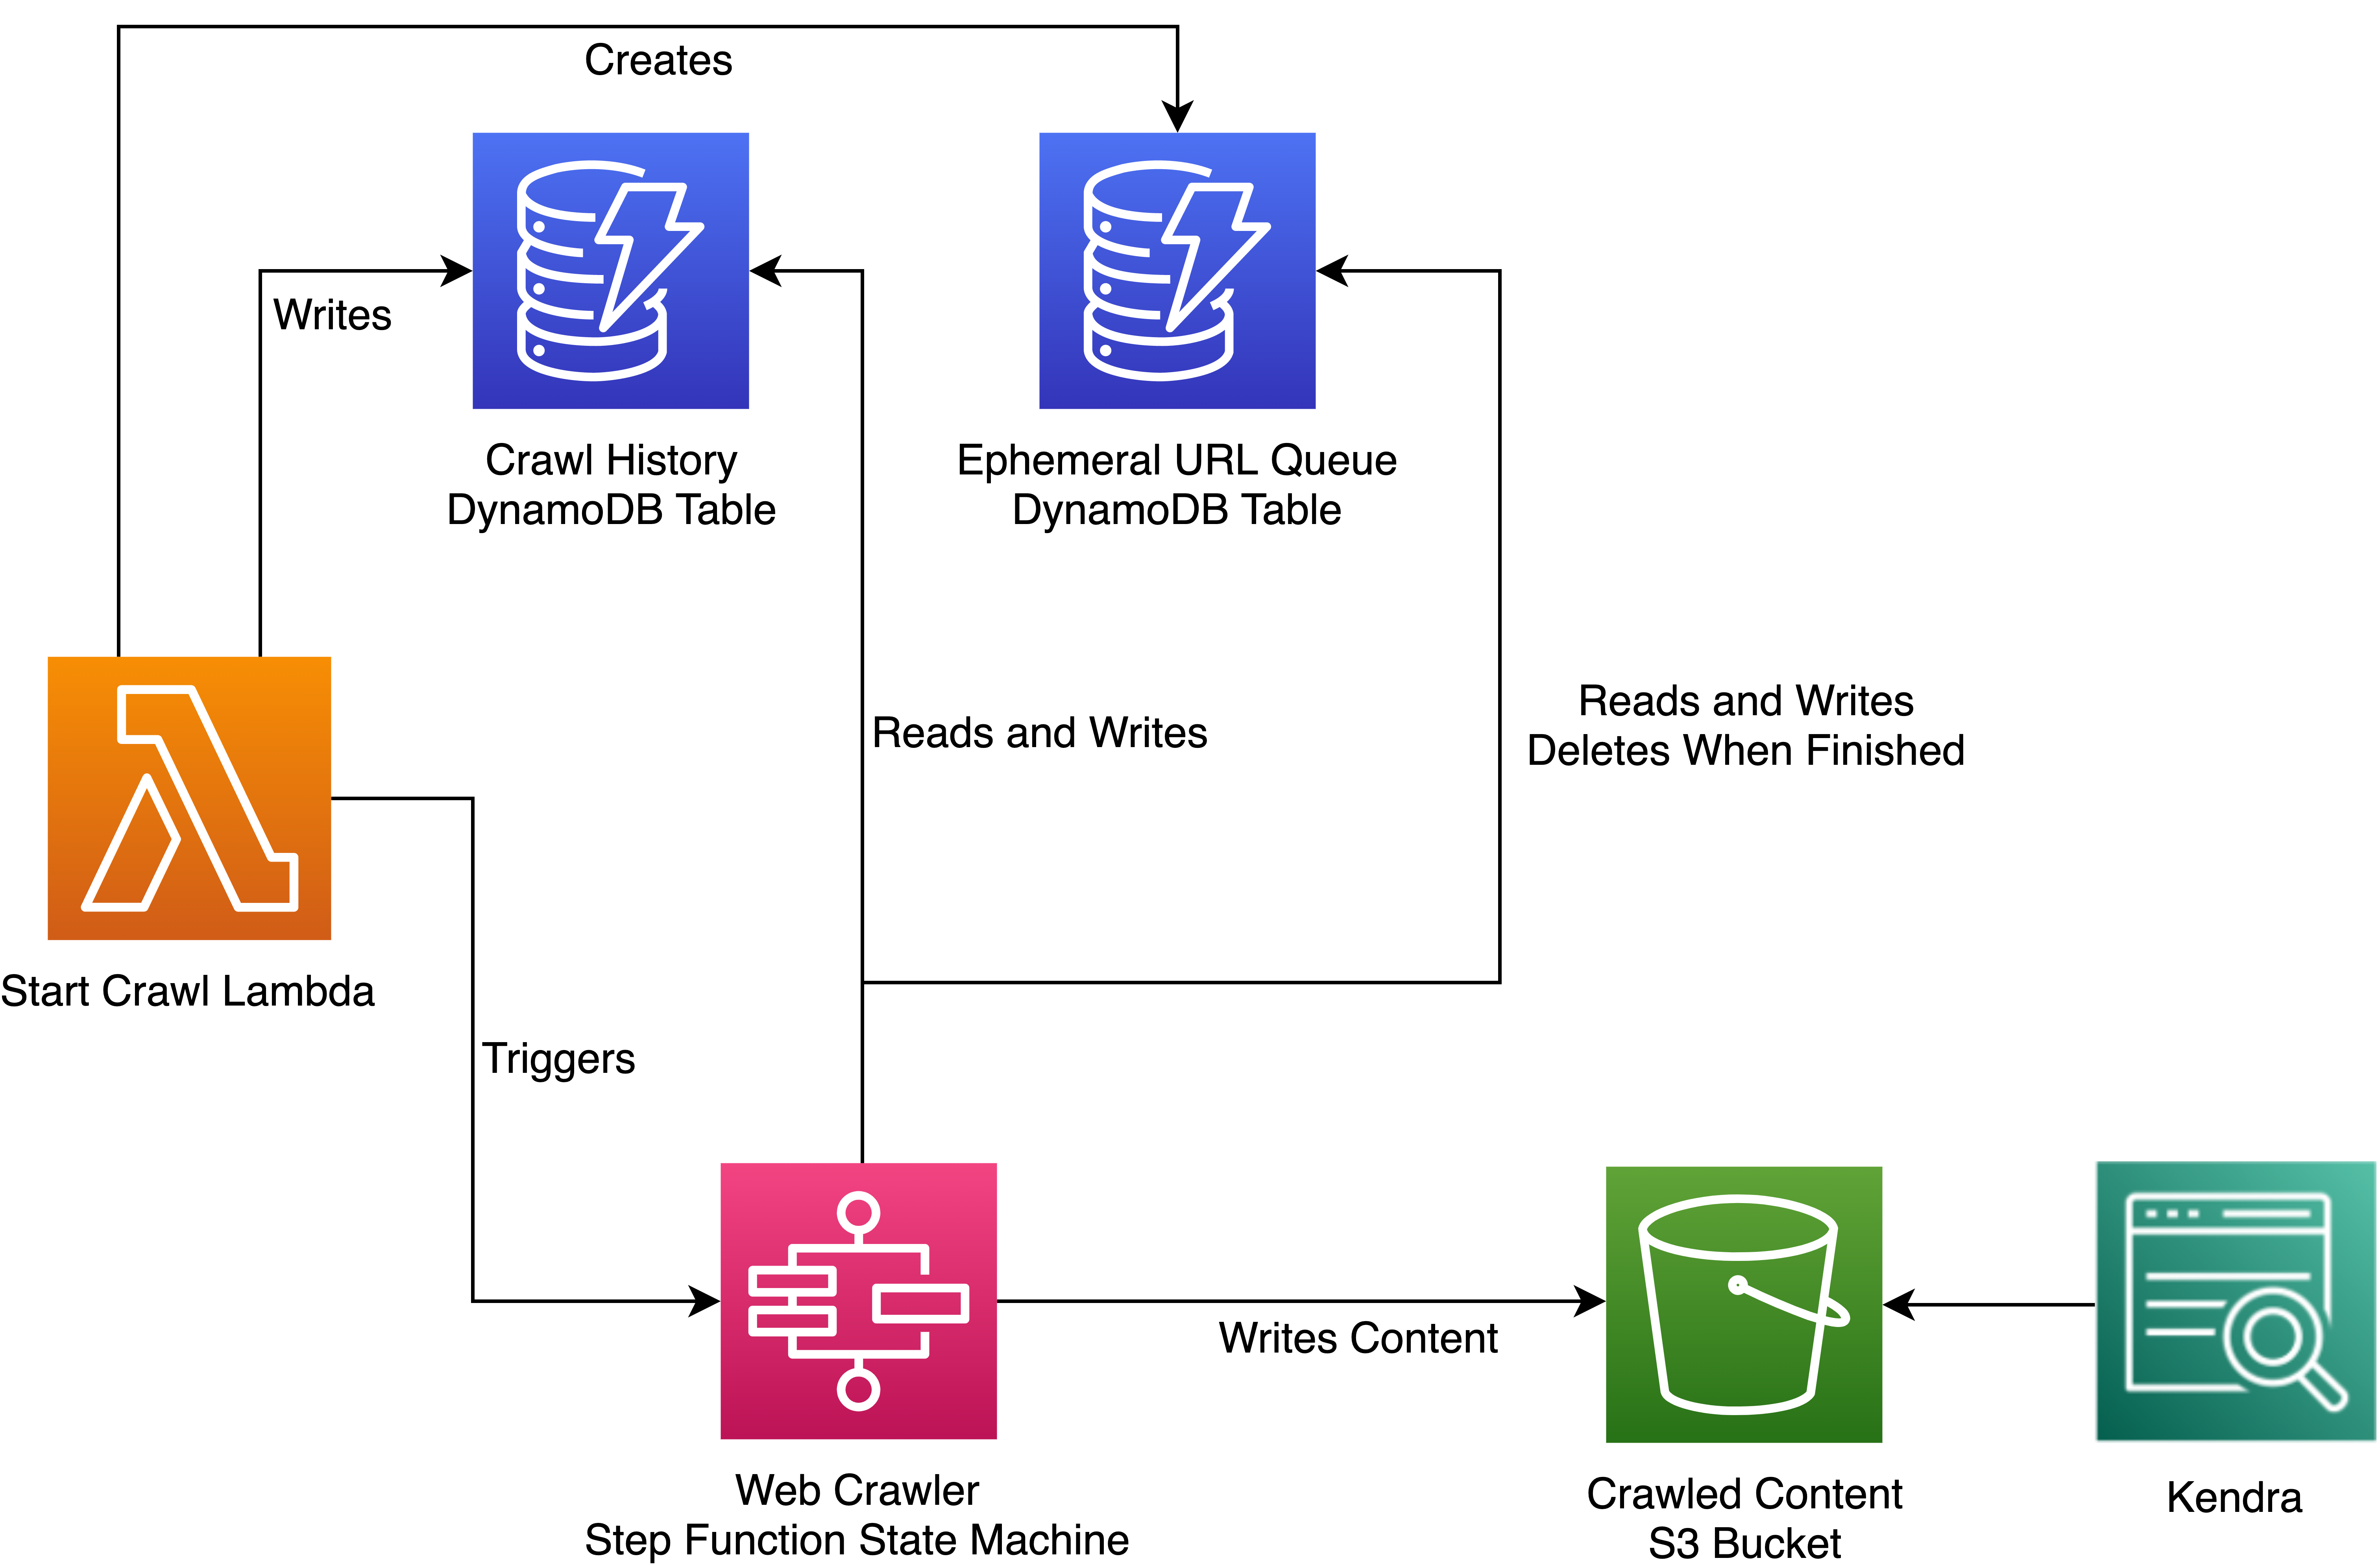
\includegraphics[width=\linewidth]{literature_review/aws_crawler_search_engine_architecture.png}
        \caption{Architecture.}
        \label{fig:aws_crawler_search_engine_architecture}
    \end{subfigure}
    \vfill
    \begin{subfigure}[t]{.9\textwidth}
        \centering
        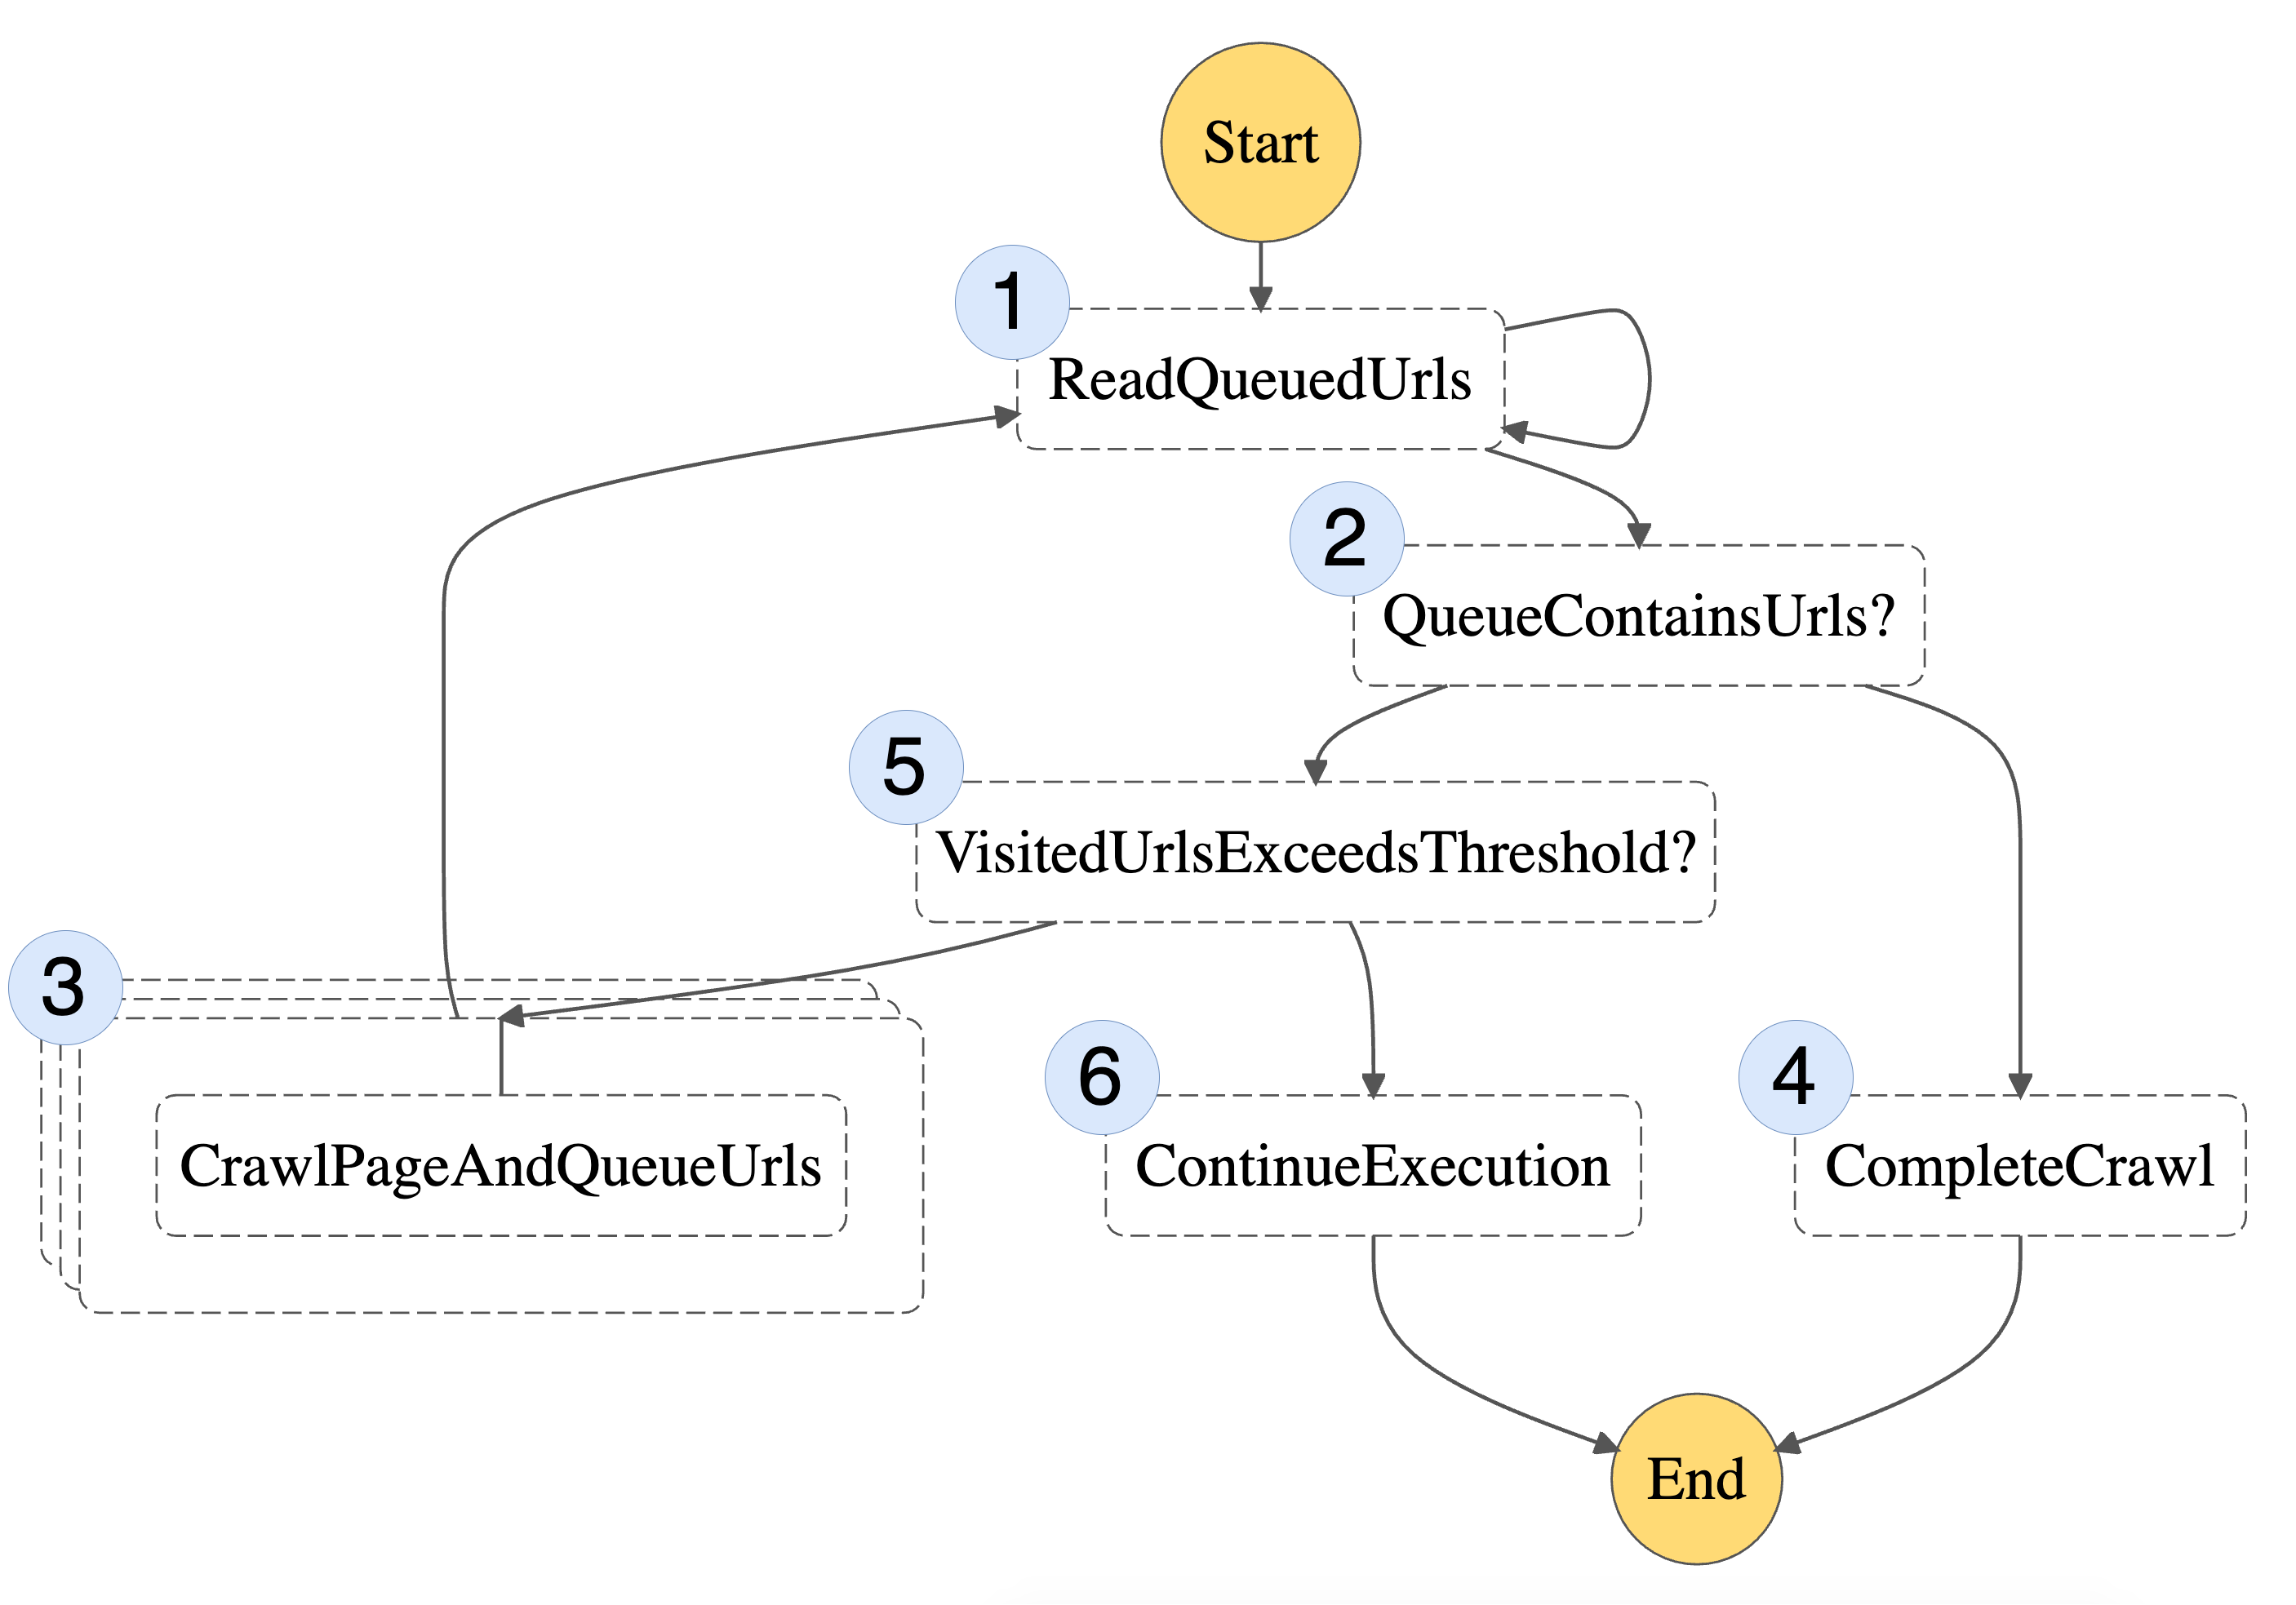
\includegraphics[width=\linewidth]{literature_review/aws_crawler_search_engine_state_machine.png}
        \caption{State machine defining web crawler algorithm.}
        \label{fig:aws_crawler_search_engine_state_machine}
    \end{subfigure}
    \caption[Example of serverless web crawler architecture]{Diagrams show the architecture and logic workflow of a serverless web crawler with a search engine. It is important to note in (b) how each step can be executed in a Lambda function dealing with a specific task so as to bypass the Lambda timeout of 15 minutes. Pictures from \citetitle{site:aws_serverless_crawler_engine_2021} \cite{site:aws_serverless_crawler_engine_2021}.}
    \label{fig:aws_crawler_search_engine}
\end{figure}

Several articles from the literature were illustrated, starting with classical web crawler solutions and ending with serverless web crawlers. Looking at Knative, there is no implementation of this type of application; the few articles mainly deal with modifying the \acrshort{KPA} autoscaling algorithm and reducing the cold start time \cite{inproceedings:knative_optimize_autoscaler_2020, article:knative_cold_start_pool_2019}.

\end{document}